\chapter{Results and Discussion}%
\label{chap:Results and Discussion}

In this chapter, the results gathered from our evaluation of the dynamic window against 
the tumbling window will be discussed by the order of the workloads. The workload 
evaluations are run multiple times for consistency of results. We will first 
discuss the workload for latency measurement, followed by periodic workload and 
finally the completeness measurement. For each workload results, we elaborate 
and discuss in details the shortcomings of the evaluation methods and the 
possible outlier situations for which the evaluation result would not agree with.



\section{Workload for latency measurement}%
\label{sec:Results Workload for latency measurement}

This workload is run with a constant low stream rate to ensure that 
the RMLStreamer is not overloaded for a more accurate latency measurement. We also measured 
CPU, throughput, and relative memory usage to determine the improvement brought by Dynamic window
in an ideal streaming environment.

For latency, Tumbling window has a median value of 1915ms, with latency ranging from 1081ms to 2624ms. 
This is as expected since the window is measured using the \emph{average} latency of all records used 
in the joined result at every \emph{trigger} event, which is fired every 2 seconds (the size of tumbling window).
In contrast, Dynamic window has sub second latency with median 57ms and ranging from 39ms to 120ms. Clearly, 
our improvement to fire the \emph{trigger} event whenever a new record arrives inside the subwindow, allows 
Dynamic window to achieve sub second latency. 

Just like latency, the throughput difference between the two windows is also significant. Dynamic window has a 
steady throughput of around 17200 records per second whereas Tumbling window fluctuates around 
12500 and 12800 records per second before stabilizing at 12750 records per second. This is expected as Dynamic 
window eventually stabilizes to a window size with the capability of processing more records than Tumbling window. This is 
due to the adjustment of window sizes at the subwindow level, allowing Dynamic window to wait for more records 
with infrequent \emph{key} attribute in the stream, before evicting the subwindow. In contrast, Tumbling window 
always evicts the content of the window after 2 seconds, even if it means that there might be more 
eligible records to be joined with the records in the soon to be evicted window, leading to lower throughput.  

Relative memory usage of Dynamic window compared to Tumbling window is similar over the lifetime of the 
evaluation run (Figure~\ref{fig:constant_mem_diff}). Dynamic window causes infrequent \emph{spikes} in memory of more 
than 100 MB memory usage than Tumbling window at certain point in the lifetime of evaluation. This can be attributed 
to the subwindows of Dynamic window growing larger than Tumbling window due to not enough records of the same 
\emph{key} attributes arriving inside the subwindows. However, Dynamic window stabilizes to a more optimal 
window size, where it uses less memory than Tumbling windows, over longer stretches of the evaluation run. At worst case, 
it uses as much memory as Tumbling window does over the course of the evaluation. 

CPU usage is higher by around 7\% for Dynamic window since it requires extra processing of the calculation of metrics. However, this 
increase in CPU usage can also be attributed to the increase in throughput, where the RMLStreamer has more joined results 
to process and map to RDF data.  

\begin{figure*}
    \begin{subfigure}[b]{0.5\textwidth}
        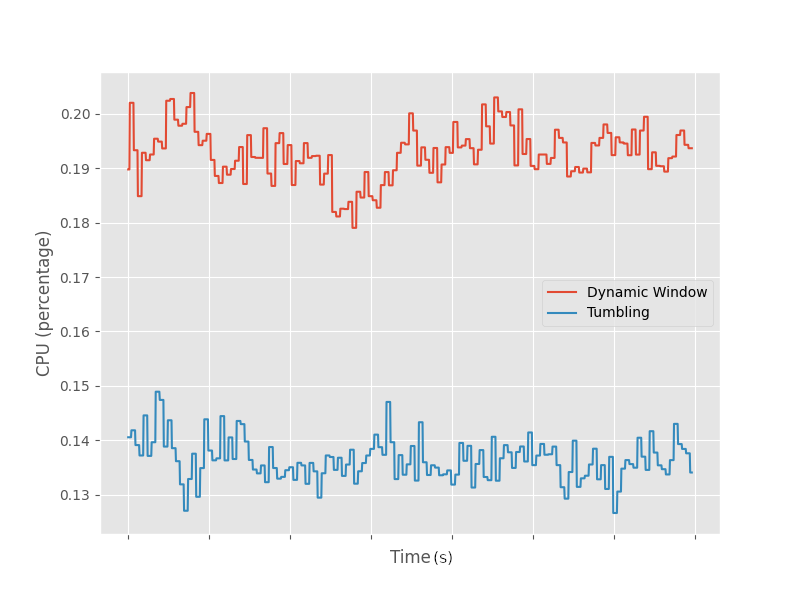
\includegraphics[width=\textwidth]{fig/constant-rate/cpu_comparison.png}
        \caption{CPU usage}
        \label{fig:constant_cpu}
    \end{subfigure}
    \hfill 
    \begin{subfigure}[b]{0.5\textwidth}
        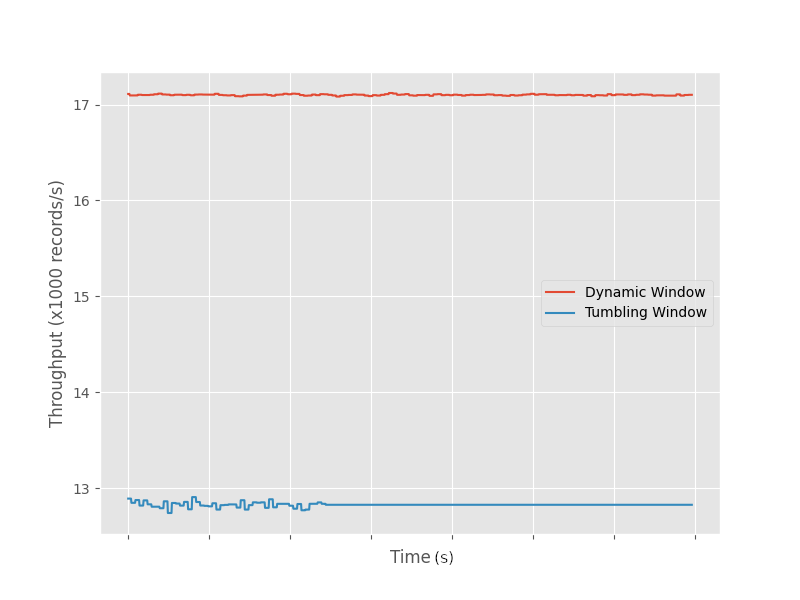
\includegraphics[width=\textwidth]{fig/constant-rate/throughput_comparison.png}
        \caption{Throughput of joined records}
        \label{fig:constant_thorughput}
    \end{subfigure}
    %%
    \begin{subfigure}[b]{0.5\textwidth}
        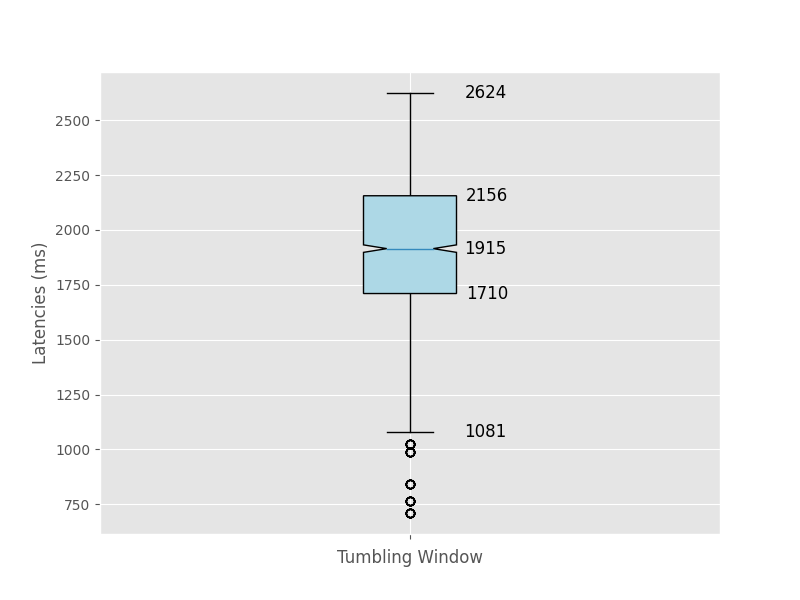
\includegraphics[width=\textwidth]{fig/constant-rate/TumblingWindow_latency_boxplot.png}
        \caption{Tumbling latency}
        \label{fig:constant_tumb_boxplot}
    \end{subfigure}
    \hfill 
    \begin{subfigure}[b]{0.5\textwidth}
        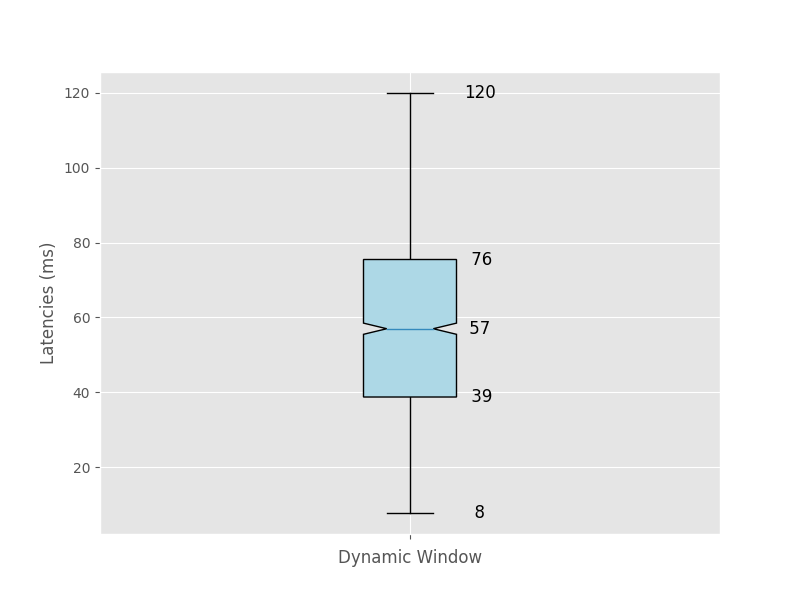
\includegraphics[width=\textwidth]{fig/constant-rate/DynamicWindow_latency_boxplot.png}
        \caption{Dynamic latency}
        \label{fig:constant_dynamic_boxplot}
    \end{subfigure}
    % 
    \begin{subfigure}[b]{\textwidth}
        \centering
        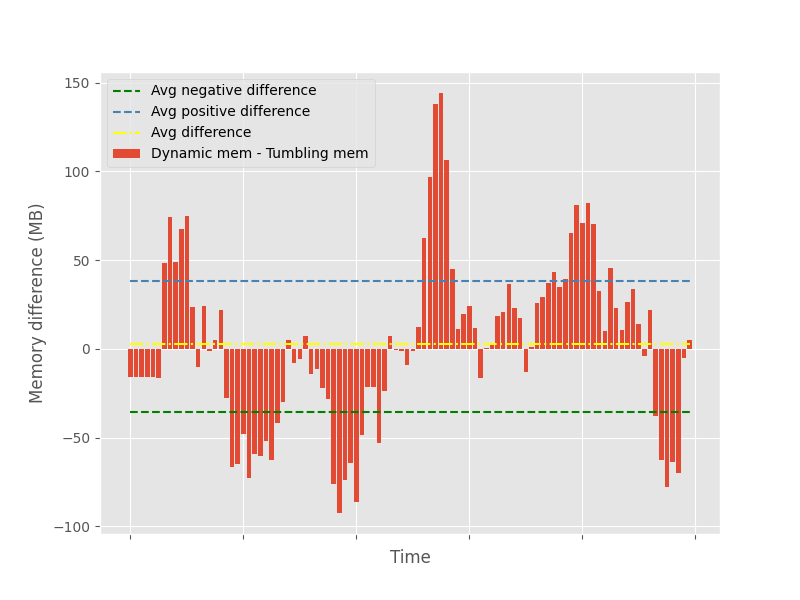
\includegraphics[width=0.5\textwidth]{fig/constant-rate/mem_difference_bar.png}
        \caption{Relative difference in memory usage from the perspective of dynamic window}
        \label{fig:constant_mem_diff}
    \end{subfigure}

    \caption{Metrics measurements for latency workload.}%
    \label{fig:constant_measurement}
\end{figure*}

\newpage
\section{Workload for periodic burst}%
\label{sec:Results Workload for periodic burst}

Dynamic window still handles the periodic burst of data with lower latency 
than Tumbling window with latency in the range from 8ms to 1669ms compared to 
Tumbling window's range from 891ms to 3904ms.
However, there is a temporary increase in latency at the beginning 
(Figure~\ref{fig:periodic_dynamic_lineplot}), 
when the burst of data arrives at every 10th second. 
This is due to the initial size of 2s subwindows for the initial low stream rate of 400 records per second. 
The subwindow sizes start to grow \textbf{larger} than 2s because of the low stream rate. 
The increase in the subwindow size results in the window 
window having more records to join; causing a back pressure to form and latency to increase.  
This results in a positive skew in the latency distribution for Dynamic window (Figure~\ref{fig:periodic_dynamic_boxplot}). 
However, Dynamic window eventually manages to shorten the subwindow sizes for adaptation to the periodic burst of data.
The shorter subwindow sizes lower the latency until it is comparable to the one achieved under the constant stream rate from the 
previous workload.


The throughput of both windows increased, as expected, compared to the workload for latency measurement 
with constant stream rate. Moreover, we observe an even bigger difference in the throughput between the 
two windows of about 7000 records per second. However, the
constant and flat throughput measurement does not agree 
with the results of ~\cite{evalution_of_spe} where there are clear "spikes" in the throughput measurement. In 
contrast to the separate evaluation of stages in ~\cite{evalution_of_spe}, 
we ran our evaluation as part of the whole RMLStreamer pipeline, from the 
ingestion of data and window joins until the generation of mapped RDF data. This causes a slight back pressure 
leading to a high and flat throughput measurement. 

CPU usage difference of the windows, is similar to the workload for latency measurement with relative increase 
in the usage to account for the processing of periodic burst of data. Dynamic window uses more CPU resources for 
calculation of metrics and dynamic adjustment of subwindow sizes. 

Surprisingly, compared with the memory usage from the workload for latency measurement, Dynamic window uses 
lesser memory of around 10 MB on average than Tumbling window, across the lifetime of the evaluation (Figure~\ref{fig:periodic_mem_diff}). 
The initial usage of the memory was higher by about 100 MB by Dynamic window due to the initial long window growth 
caused by the low stream rate. However, once 
the dynamic adjustment of subwindow kicks in, it reduces the memory usage even when there is a burst of data. The subwindow size
is adjusted to be small to frequently evict the records inside the window. 

\begin{figure*}
    \begin{subfigure}[b]{0.5\textwidth}
        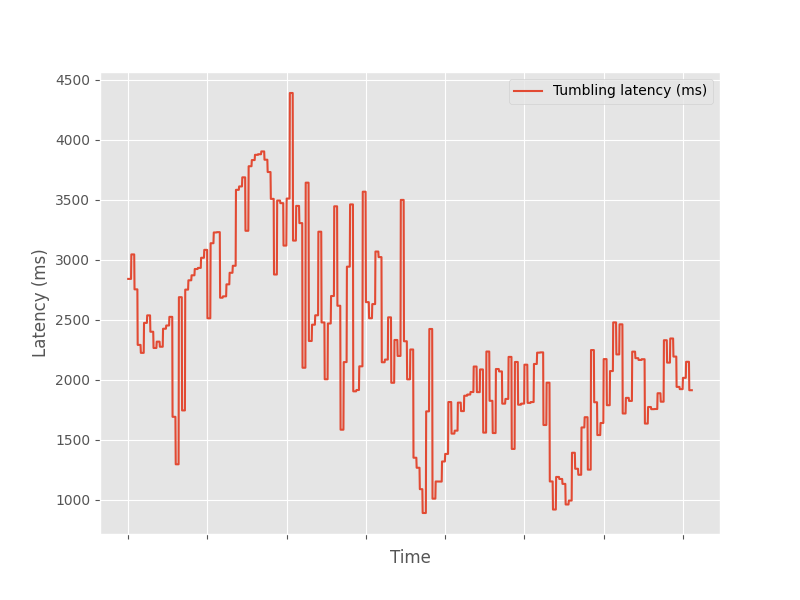
\includegraphics[width=\textwidth]{fig/periodic/Tumbling_latency_lineplot.png}
        \caption{Tumbling latency }
        \label{fig:periodic_tumbling_lineplot}
    \end{subfigure}
    \hfill
    \begin{subfigure}[b]{0.5\textwidth}
        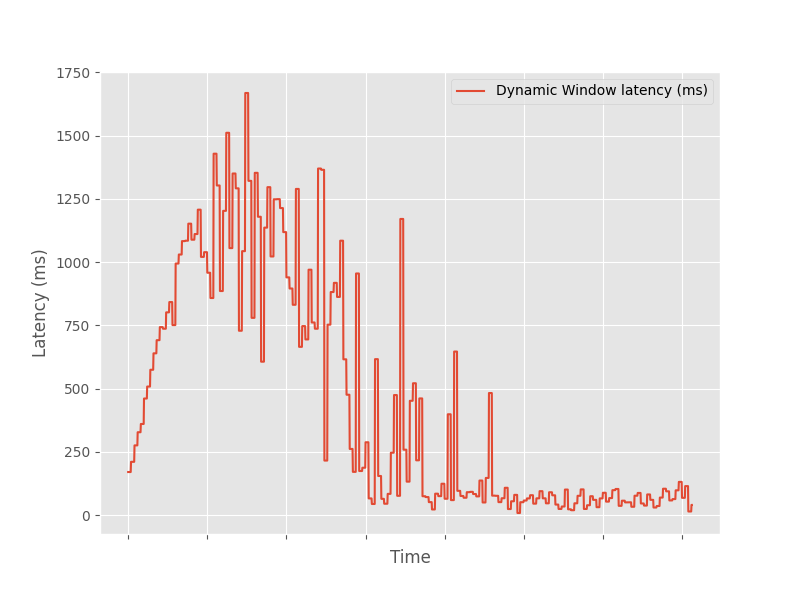
\includegraphics[width=\textwidth]{fig/periodic/DynamicWindow_latency_lineplot.png}
        \caption{Dynamic latency }
        \label{fig:periodic_dynamic_lineplot}
    \end{subfigure}
    \caption{Latency measurement of periodic workload over the lifetime of evaluation}
    \label{fig:periodic_latency_lineplot}
\end{figure*}

\begin{figure*}
    \begin{subfigure}[b]{0.5\textwidth}
        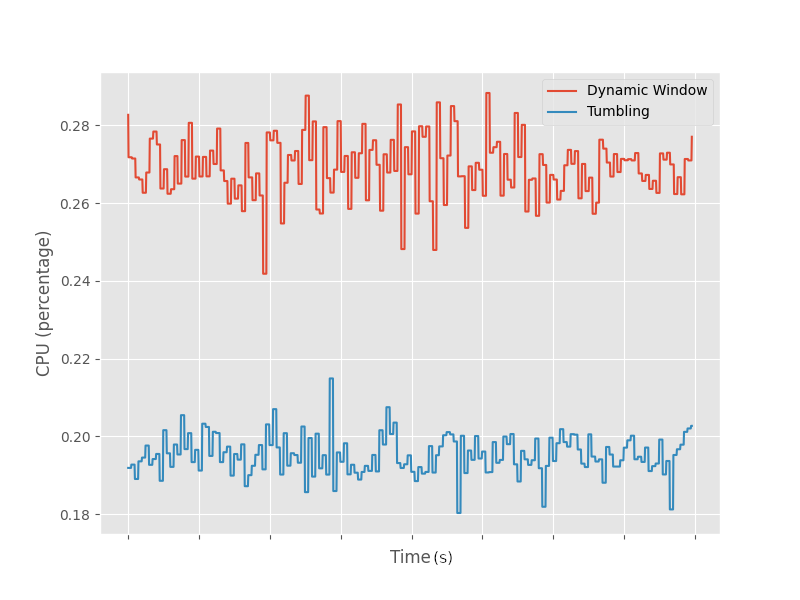
\includegraphics[width=\textwidth]{fig/periodic/cpu_comparison.png}
        \caption{CPU usage}
        \label{fig:periodic_cpu}
    \end{subfigure}
    \hfill 
    \begin{subfigure}[b]{0.5\textwidth}
        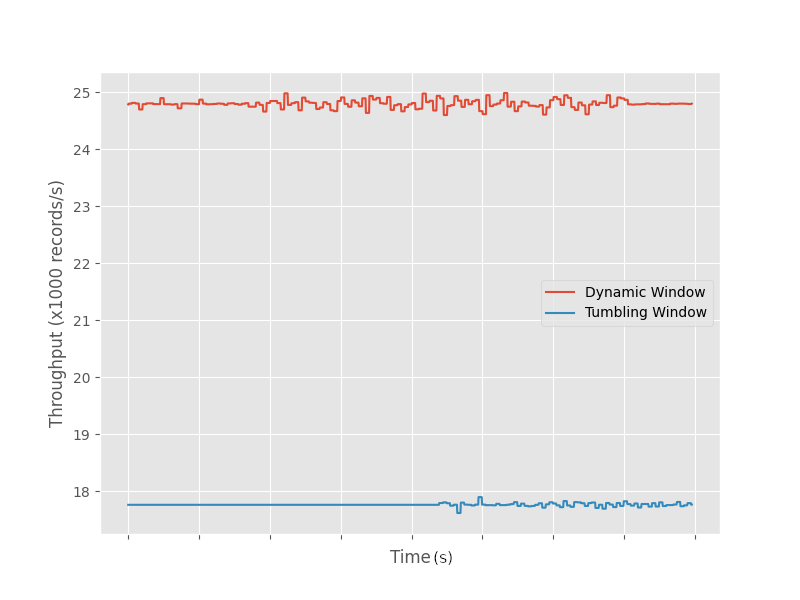
\includegraphics[width=\textwidth]{fig/periodic/throughput_comparison.png}
        \caption{Throughput of joined records}
        \label{fig:periodic_throughput}
    \end{subfigure}
    %%
    \begin{subfigure}[b]{0.5\textwidth}
        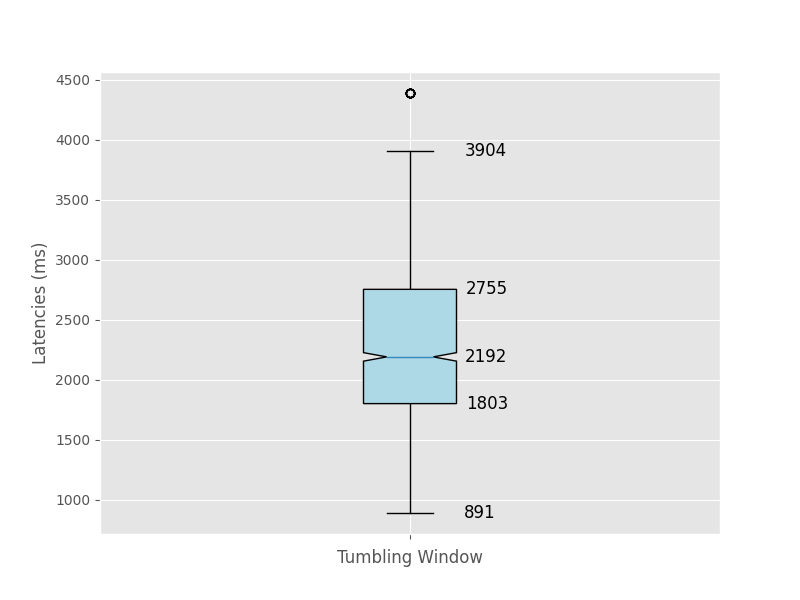
\includegraphics[width=\textwidth]{fig/periodic/TumblingWindow_latency_boxplot.png}
        \caption{Tumbling latency distribution}
        \label{fig:periodic_tumb_boxplot}
    \end{subfigure}
    \hfill 
    \begin{subfigure}[b]{0.5\textwidth}
        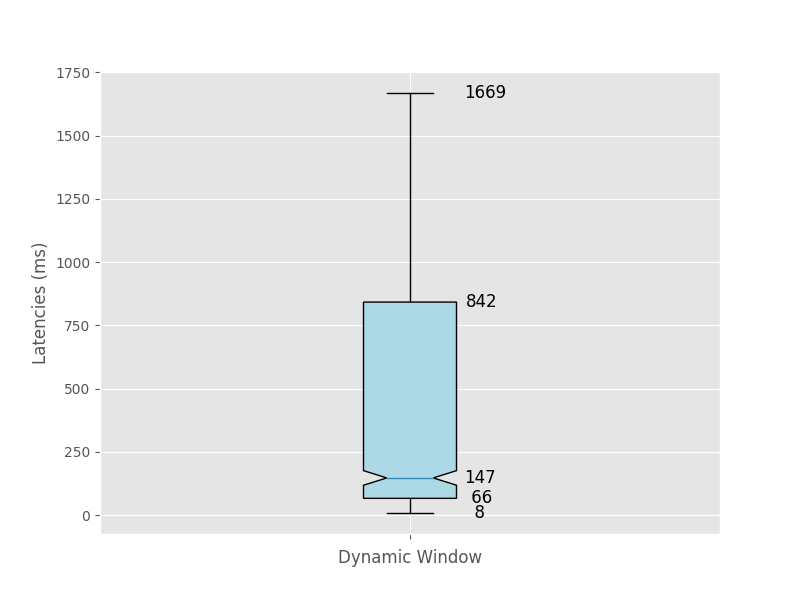
\includegraphics[width=\textwidth]{fig/periodic/DynamicWindow_latency_boxplot.png}
        \caption{Dynamic latency distribution}
        \label{fig:periodic_dynamic_boxplot}
    \end{subfigure}
    % 
    \begin{subfigure}[b]{\textwidth}
        \centering
        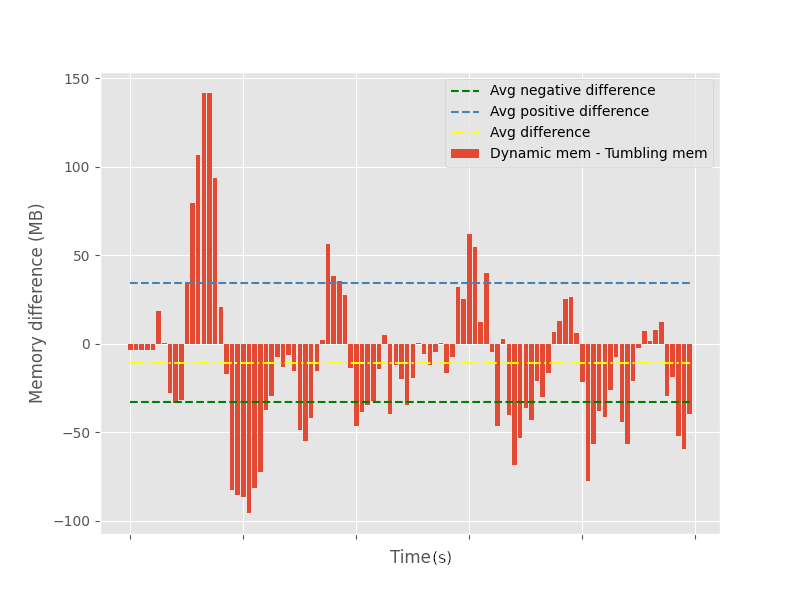
\includegraphics[width=0.5\textwidth]{fig/periodic/mem_difference_bar.png}
        \caption{Relative difference in memory usage from the perspective of dynamic window}
        \label{fig:periodic_mem_diff}
    \end{subfigure}

    \caption{Metrics measurements for periodic workload.}%
    \label{fig:periodic_measurement}
\end{figure*}

\newpage
\section{Workload for completeness measure}%
\label{sec:Workload for completeness measure}

From the results in Table~\ref{tab:dynamic_completeness}, and 
Table~\ref{tab:tumbling_completeness}, we could conclude that Dynamic window 
outperforms Tumbling window in terms of generating a more \emph{complete} output. 
Dynamic window has an IOU score of \textbf{1} for constant low stream rate
due to the subwindow sizes growing large 
enough to accommodate all the required records, to generate the \emph{complete} set 
of output. In contrast, Tumbling window scores only \textbf{0.749}, leading to 
a conclusion that a window size of 2s is not enough to process the low stream rate 
of the evaluation data. 

Similary for periodic burst input, Dynamic window outperforms Tumbling window with a
score of \textbf{0.982} whereas Tumbling window only scores \textbf{0.780}. The high IOU 
score of Dynamic window could be explained by its ability to adapt the window sizes according 
to the changing stream rate to hold enough records for maximal joined output generation; moreso 
than Tumbling window. 


\begin{table}[htbp]
    \centering
    \resizebox{\textwidth}{!}{%
\begin{tabular}{|r|r|r|r|r|}
\hline
\multicolumn{1}{|c|}{Stream rate} & \multicolumn{1}{c|}{Generated (triples)} & \multicolumn{1}{c|}{Expected (triples)} & \multicolumn{1}{c|}{Common (triples)} & \multicolumn{1}{c|}{\textbf{IOU score}} \\ \hline
Constant rate                     & 30,771,450                               & 30,771,450                              & 30,771,450                            & \textbf{1}                              \\ \hline
Periodic burst                    & 31,753,420                               & 32,319,110                              & 31,753,420                            & \textbf{0.982}                          \\ \hline
\end{tabular}%
}
\caption{Dynamic window's completeness measurement. The \emph{Expected (triples)} are the number of triples generated by the 
bounded data processing RMLStreamer.}
\label{tab:dynamic_completeness}
\end{table}

\begin{table}[htbp]
    \centering
    \resizebox{\textwidth}{!}{%
\begin{tabular}{|r|r|r|r|r|}
\hline
\multicolumn{1}{|c|}{Stream rate} & \multicolumn{1}{c|}{Generated (triples)} & \multicolumn{1}{c|}{Expected (triples)} & \multicolumn{1}{c|}{Common (triples)} & \multicolumn{1}{c|}{\textbf{IOU score}} \\ \hline
Constant rate                     & 23,059,350                               & 30,771,450                              & 23,059,350                            & \textbf{0.749}                              \\ \hline
Periodic burst                    & 24,412,150                               & 31,287,300                              & 24,412,150                            & \textbf{0.780}                          \\ \hline
\end{tabular}%
}
\caption{Tumbling window's completeness measurement. 
    The \emph{Expected (triples)} are the number of triples generated by the 
bounded data processing RMLStreamer.}
\label{tab:tumbling_completeness}
\end{table}


\section{Summary}%
\label{sec:Result Summary}

In summary, these results show that our implementation of Dynamic window 
provides lower latency, higher throughput, and a more complete 
output than Tumbling window for both 
workloads of constant stream rate, and unstable periodic burst stream rate.
This validates three of our hypotheses that Dynamic window would outperform 
windows of fixed sizes in those three areas. 

Although memory usage dropped in the workload with periodic burst rate, we 
could not confidently conclude that the Dynamic window effectively used lesser memory
on average than Tumbling window. The measurement was based on the heap memory of the 
whole evaluation job, not just the window operator. Therefore, there is a need for a 
more precise measurement of memory usage. For example, by counting the number of 
records that effectively reside in the windows at any moment. This approach is currently 
limited since Flink does not expose API to count the number elements residing 
in its default implementation of Tumbling window.  

The results for throughput also deviate from those reported by Van Dongen and Van den Poel(2020)~\cite{evalution_of_spe}. 
This could be explained by the fact that we ran the evaluation using the whole pipeline of RMLStreamer, including 
the stage where the joined results are mapped to RDF data. This incurs some back pressure from the mapping stage, 
causing the throughput of the join stage to stay constant and flat.    

Overall, we could conclude that Dynamic windowing is viable to replace the fixed size windows. Especially in use 
cases, where windows are not required to be of fixed size with variable stream rate.  

